\section{Multifrequency Multistage Radiolocation System}
\label{sec:mfms}
    This section explains \gls{mfms} in greater detail.
    Akin to other \gls{firl}s, \gls{mfms} consists of two main phases.
    During the offline phase, \gls{rss} information from anchor nodes is collected at many locations in the environment and used to approximate the radio wave propagation function.
    The online phase, on the other hand, makes use of the approximated propagation function obtained in the former phase.
    %  is used for localization purposes with new observations obtained at arbitrary locations.
    However, one major difference between \gls{mfms} and conventional \gls{firl} approaches is that \gls{mfms} employs three types of radio setups in three different stages to infer the location of the agent.

    \begin{figure}[thpb]
        \centering
        \includegraphics[width=\linewidth]{figures/rss-vs-distance.jpg}
        \caption{\label{fig:log-distance}RSSI readings of NLoS and LoS APs acquired with a stationary agent}
    \end{figure}

    The main motivation behind employing multisource information is to exploit the diversity of the propagation characteristics of the different frequencies.
    As can be seen in the \Cref{eq:log-distance} and \Cref{fig:log-distance}, the received power and separation distance shows a log-linear relationship.
    %  demonstrates the log-distance relationship between received power and the separation between two antennas in two different frequencies in \gls{uhf} radio band.
    This figure implies two fundamental problems in radiolocation systems:
    The first problem is that as the carrier frequency increases path loss increases significantly, which limits the radio covarage and localization ability of the system in large environments.
    On the other hand, as the carrier frequency increases, the separation between two antennas, i.e.\ the anchor node and the target to be localized, can be identified with finer spatial resolution.
    Therefore, the trade-off between radio coverage and spatial localization resolution can be resolved by employing different frequencies in indoor localization systems by fusing the information acquired from the anchor nodes using different carrier frequencies.
    Thus, \gls{mfms} employs a \gls{lora} (900 MHz), a WiFi \gls{ap} and a Bluetooth (2.4 GHz) beacon in each anchor node.
    \Cref{tab:specs} tabulates the specifications of the radios consisting in each anchor node, while \Cref{fig:module} demonstrates the details of the anchor nodes.
    In detail, wider spatial coverage is achieved by using \gls{lora} modules working at 900 MHz while finer spatial resolution provided by WiFi and Bluetooth both working at 2.4 GHz frequency.

    \begin{table}
    \begin{center}
    \caption{\label{tab:specs}The specifications of radios used in anchor nodes}
      \begin{tabular}{@{}lccc@{}}\toprule[1.5pt]
        Property                        &WiFi           &Bluetooth      &\gls{lora}\\ \midrule[1.5pt]
        Frequency [MHz]:                &2400           &2400           &900 \\ \midrule
        Communication Bandwidth:        &1-11 Mbps      &Upto 4 Mbps    &10 Kbps \\ \midrule
        Transmission Power $P_t$ [dBm]: &17             &10             &24 \\ \midrule
        Reciever Sensivity [dBm]:       &?              &-98            &-101 \\ \midrule
        Communication Range [m]:        &$<$20          &$~$10            &$>$100  \\\bottomrule[1.5pt]
      \end{tabular}
    \end{center}
    \end{table}

    \begin{figure}[thpb]
       \centering
       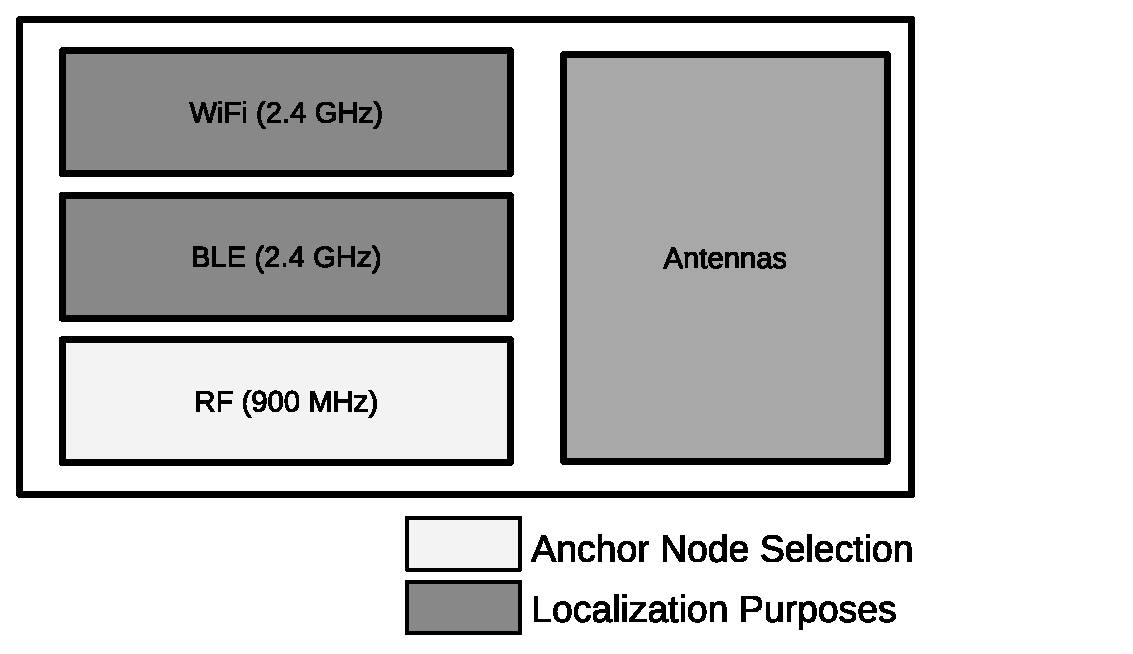
\includegraphics[width=\linewidth]{figures/mfms_module.eps}
       \caption{\label{fig:module}\gls{mfms} Anchor Nodes}
    \end{figure}

    \subsection{Spatially-coherent Path Loss Exponent Estimation}
    This section covers the details of the joint path loss exponent estimation which forms the first stage of \gls{mfms}.
    We approach the \gls{firl} problem in the scope of curve fitting.
    However, unlike many approaches proposed mentioned earlier, \gls{mfms} does not try to blindly fit a function which best explains the training data given the location labels.
    Moreover, \gls{mfms} does not consider the path loss exponent as a variable describing the whole localization environment.
    Instead, we approach the problem as curve fitting for path loss exponent differing in value depending on the regions at which the agent resides.
    In other words, the path loss exponent for \gls{mfms} is a function of both location.
    Therefore, the proposed system is able account for non-uniform distribution of obstructions in space.

    \begin{figure}[thpb]
       \centering
       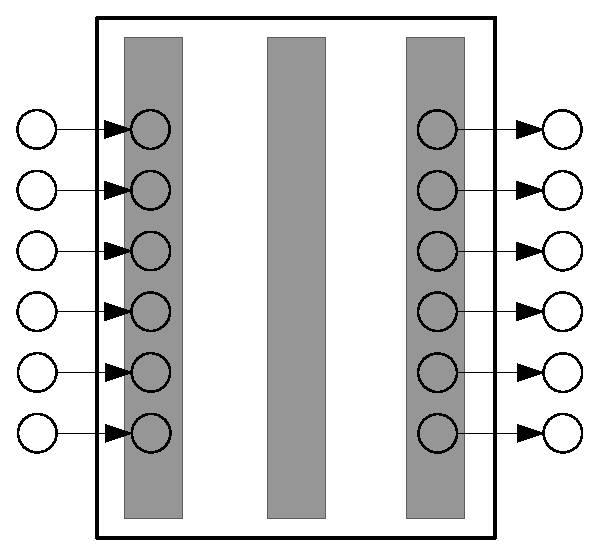
\includegraphics[width=\linewidth]{figures/softmax.eps}
       \caption{\label{fig:softmax}The softmax classifier assigns weights for each anchor node based on the evidence representing the probability of residing in a grid cell $g$.}
    \end{figure}

    Let $\Omega=\{g_i | i=1\ldots n_{grid}\}$, is the localization environment which is divided into $n_{grid}$ number of grids $g$.
    An arbitrary position $\bm{x} \in \Omega$ can be in a shadowed region for any anchor node; thus, \gls{mfms} selectively chooses which anchor nodes to use to localize the agent in $\Omega$.
    This selection is performed by mapping the measurement vector acquired at time step $k$ $\bm{m}^{k}_j \in \mathbb{Z}^{n_{node}}$ with a set of weights $\bm{w}_g \in \mathbb{R}^{n_{node}}$ such that $\sum_g \bm{w}_g = 1$.
    The weights of each grid is learned with a softmax classifier, which is depicted in \Cref{fig:softmax}.
    The classifier is solely based on \gls{lora} measurements due to the higher probability of observing multiple \gls{lora} modules in arbitrary positions in the environment, thanks to the smallar path loss they introduce.
    \Cref{eq:weighted_m} shows the result of the selection process.

    \begin{equation}
        \label{eq:weighted_m}
        \bm{\widetilde{m}}^{k}_j = \bm{w}_g \bm{m}^{k}_j
    \end{equation}

    For each anchor node, the path loss exponent is estimated with \gls{ldpl} model in a least square sense.
    The estimated spatially-coherent path loss exponent, a set physical parameter defining the radio wave propagation, is incorporated into the location estimation process explained in Stage-II\@.

    \begin{equation}
        n^{*,i}_g = \argmin_n{\sum_j \left(\norm{\bm{x}_g}_2 - f_d(m^i_{j_g},n)\right)^2}
    \end{equation}
    where $\bm{x}_g$ and $m^i_{j_g}$ denote the center position of grid $g$, and measurements acquired in grid $g$, while $f_d(\cdot)$ denotes \gls{ldpl} model.

    \subsection{Pinpoint Localization}
    This section gives details of the second stage of the \gls{mfms} which is the pinpoint localization.
    After localizing the agent in grid-level and selecting which anchor nodes to be employed, the propagation function $\hat{g}_d(\cdot)$ can be formulated as below:
    % , which $\mathbb{Z}^{n_{node}\times n_m} \mapsto \mathbb{R}^2$:
    % Similar to \gls{ldpl}, our radio wave function approximation is given below:
    \begin{equation}
        \label{eq:propfunct}
        \hat{g}_d(\bm{\widetilde{m}}^{k-n_{m}:k}_j, \bm{n}^*_g)= \bm{\hat{x}}
    %   n(k,t)^* = \argmin_n \bm{e}^i  = \argmin_n \{d^i_j - \hat{f}^i_d(m_i, n, t)\}
    \end{equation}
    where $\bm{\widetilde{m}}^{k-n_{m}:k}_j$, $\bm{n}^*_g$, and $\bm{\hat{x}}$ are the weighted measurement vector between time steps $k-n_m$ and $k$, the estimated path loss exponent vector of each anchor node for grid $g$ and the estimated absolute position of the agent, respectively.
    As can be seen in \Cref{eq:propfunct}, the propagation function incorporates the weighted measurements with the spatially- and temporally-coherent path loss exponent so that the physical characteristics of the radio waves, represented with the path loss, are enforced into the model as a parameter.

    \begin{figure}[thpb]
       \centering
       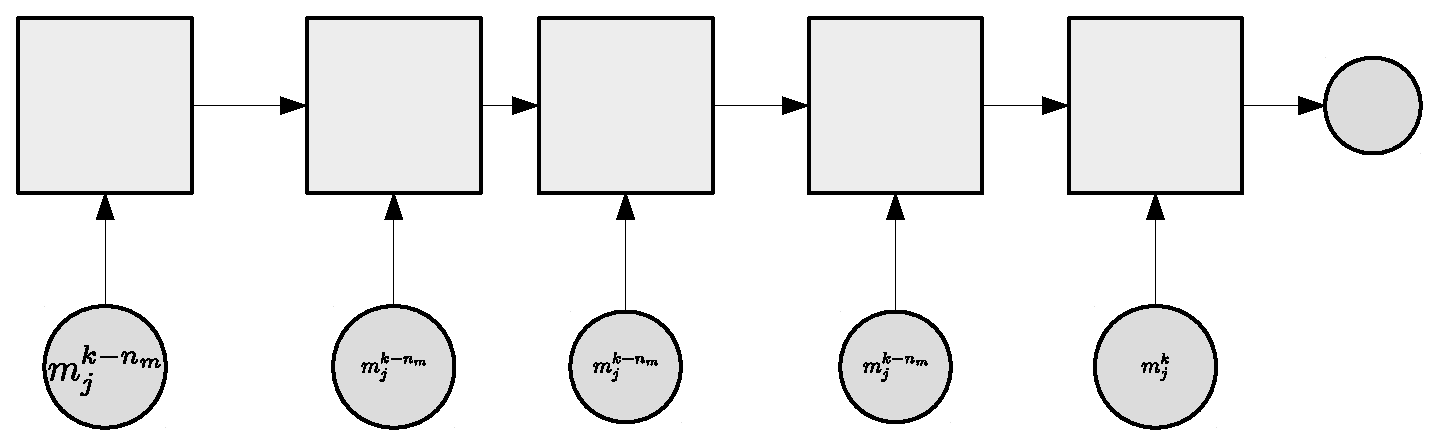
\includegraphics[width=\linewidth]{figures/gru.eps}
       \caption{\label{fig:gru}GRU}
    \end{figure}

    The propagation function of WiFi $\hat{g}^w_d(\cdot)$ and Bluetooth $\hat{g}^b_d(\cdot)$ anchors are approximated with two separate recurrent neural networks, consisting of three layers of \gls{gru}~\cite{cho2014learning}.
    These functions are attained with a \gls{sgd} based back-propagation algorithm.
    After approximating the propagation functions, these are employed to estimate the location of the agent.
    Specifically, the pinpointing algorithm incorporates the spatially-coherent path loss exponent along with the weighted measurements to estimate $\bm{\hat{x}}^w$ and $\bm{\hat{x}}^b$, estimated positions by using WiFi measurements and Bluetooth measurements, respectively.

    \Cref{fig:gru} depicts the Stage-II of \gls{mfms} in an unfolded representation.
    % The locatization environment is divided into $n_{grid}$ number of grids in order to obtain


    \subsection{Information Fusion}
    This section of the paper further explains the Stage-III of the \gls{mfms}.
    The Stage-III is essentially an information fusion layer of the model where location estimates of WiFi and Bluetooth measurements are fused into one final entity.
    The incorporation of two estimates are achieved in the framework of a \gls{nn} consisting of 3 layers.
    The network is in a gradually narrowing structure such that the first, second and last layer contain 8, 4, 2 neurons, respectively.
    \Cref{fig:fusion} demonstrates the Phase-III\@.

    \begin{figure}[thpb]
       \centering
       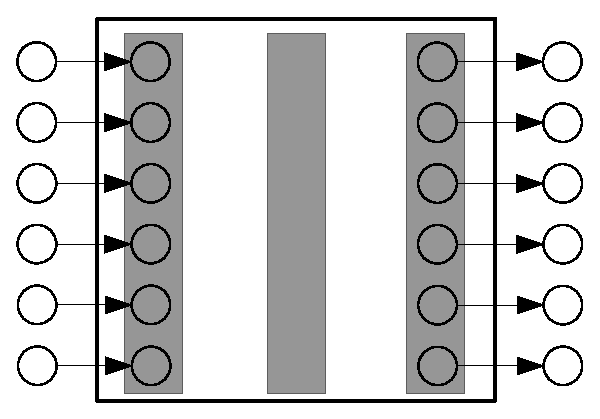
\includegraphics[width=0.95\linewidth]{figures/fusion.eps}
       \caption{\label{fig:fusion}Two location estimates of WiFi and Bluetooth approximations are fused with a 3 layered-\gls{nn}.}
    \end{figure}
